\part{Desarrollo}


\section{Diseño de los algoritmos}
\subsection{Test de primalidad}
Según el Teorema fundamental de la aritmética, todo entero positivo mayor que $1$1 es un número primo o bien un único producto de números primos, es decir, que un número natural es primo si y sólo si es divisible únicamente por sí mismo y por $1$.\\
Por lo tanto, la forma más sencilla de comprobar si un número es primo es comprobar si es divisible por cualquier número natural de $2$ a $n-1$.\\
\\
Sin embargo, no hace falta probar todos los números naturales hasta $n-1$. Al encontrar un divisor $p$ de $n$, en realidad estamos encontrando también el divisor $q$, ya que $n / p = q$. Pongamos que $n$ es el cuadrado de $p$, es decir, $n = p \times p \Rightarrow p = \sqrt{n}$. Como estamos probando números naturales de menor a mayor, cualquier número $q > p$ que también sea divisor de $n$ ya habría sido detectado anteriormente. Por lo tanto, no es necesario probar números superiores a $\sqrt{n}$. Como estamos trabajando con números naturales, aplicaremos la función suelo a la raíz cuadrada, ya que si $p \leq \sqrt{n} \rightarrow p \leq \left \lfloor \sqrt{n} \right \rfloor \leq \sqrt{n} \leq \left \lceil \sqrt{n} \right \rceil \Rightarrow p \leq \left \lfloor \sqrt{n} \right \rfloor$.\\
Otra optimización es, en el caso de que $n$ no sea par, saltarnos los números pares.\\
\\
Por lo tanto, el algoritmo diseñado para comprobar si un número natural $n$ es primo o compuesto es el siguiente:
\begin{enumerate}
    \item Si $n$ es divisible entre $2$, es compuesto.
    \item Por cada número natural \textit{impar} $p \in [3, \left \lfloor \sqrt{n} \right \rfloor]$:
    \begin{enumerate}
        \item Si $n$ es divisible por $p$, es compuesto.
    \end{enumerate}
    \item En cualquier otro caso, es primo.
\end{enumerate}

La implementación usada, en C++, se puede encontrar en \href{run:./src/primes/primes.hpp}{\texttt{src/primes/primes.hpp}} (función \texttt{is\_prime}).

\section{Implementación}
\subsection{Tests Funcionamiento }
Para comprobar el correcto funcionamiento de los algoritmos implementados, se han llevado a cabo una batería de tests, tanto para verificar que los resultados obtenidos son correctos, como para poder evaluar el rendimiento de ejecución para differentes tamaños de números


\subsubsection{Test funcionales}

Con estos test lo que se busca es probar que el algoritmo desarrollado funciona correctamente para ello se ha prubado a ejecutar con números que previamente se conoce si son primos o no. En todos los casos se han obtenido resultados correctos por lo que se puede concluir que funciona correctamente
\begin{figure}[H]
			\makebox[\textwidth][c]{
\includegraphics[width=5cm]{img/uc3m_logo.png}}
\end{figure}
  

\section{Evaluación analítica}
\subsection{Test de primalidad}

Teniendo en cuenta el algoritmo descrito anteriormente, podemos calcular analíticamente el coste del mismo.\\
Asumiendo cualquier coste no dependiente del tamaño del número de entrada $n$ como constante, el coste del algoritmo viene derivado del paso 2, el cual es un bucle que se repite en el peor de los casos $(\left \lfloor \sqrt{n} \right \rfloor - 3)/2$ veces, por lo que podemos decir que la complejidad temporal es:
\begin{equation}
    T(n) = \frac{\left \lfloor \sqrt{n} \right \rfloor - 3}{2}
\end{equation}

La memoria es independiente del tamaño del problema, por lo que la complejidad temporal es:
\begin{equation}
    S(n) = 1
\end{equation}



\section{Evaluación empírica}

Para evaluar el rendimeinto, se ha ejecutado el programa en todo el rango de valores posibles que permite el sistema, desde números unidígito, hasta lo máximo posible que permite el sistema, en este caso números de 20 digitos. Para obtener dicho número máximo, se emplea la variable \texttt{MAX\_UINT} que retona el mayor número posible de computa en C++.\\
\\
Para cada longitud de numeros se calculan un total de 900 numeros aleatorios y se aplica la función a cada uno de ellos para saber si es primo, de tal forma que se obtiene la media de tiempo de ejecución para dicha longitud de número, de esta manera se busca obtener resultados lo más fiable posibles.\\


Una vez obtenidos los resultado indicados previamente, se guardan en formato CSV y se representan gráficamente mediante la librería 'matplotlib'. Dicha representacion gŕfica resulta de gran utilidad para comprobar como el tiempo de ejecución se mantiene etable con pequeñas variaciones para número de hasta 15 digitos, de ahí en adelante se aprecia que acada aumento de tamaño de número se trduce en un aumento cada vez más significativo en el tiempo de ejecución 

\begin{figure}[H]
	\makebox[\textwidth][c]{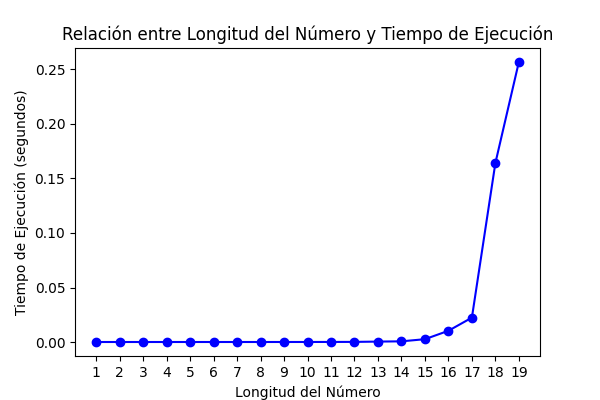
\includegraphics[width=15cm]{img/scatter_plot_primes.png}}
\end{figure}

\newpage